% Provenance (never printed): see sources/outline_sources.md (Year 3: the main
% field and its secular variation, rock magnetism, palaeomagnetic poles, apparent
% polar wander, magnetostratigraphy, the geodynamo). Brief: sources/book5/BRIEFS.md,
% ch. 4. Curves and maps from figdata/bachelor-3/igrf_field.py (IGRF-14),
% palaeomag_stats.py (the invented Kesta terrane, its Fisher statistics, the
% Zijderveld specimen and the reference APW path), magnetostratigraphy.py.
% Exercise and problem values in the Book 5 scratch calculator calc/ch04.py.
\chapter{Geomagnetism and Palaeomagnetism}\label{ch:b3:palaeomagnetism}

A basalt flow erupted sixty million years ago cooled with its tiny grains of
magnetite locked parallel to the field of the day. Drilled today, oriented in
place, sliced into small cylinders and heated
step by step in a room shielded from the present field, it still says how far
it then lay from the pole and which way it faced. Thousands of such
measurements, from every continent and every age, have told how the continents
moved before the ocean floors that record their motion were born, and in
which order the field has reversed through the layers of a sedimentary
section. This chapter describes the field as it is today, how rocks record it,
how a direction is extracted and averaged, and what a palaeomagnetic pole says
about the motion of a plate.

\begin{recall}
The Earth as a magnet and the magnetic declination are in the physics books'
school volumes; magnetic domains, hysteresis, remanence and the Curie
temperature in their Year 3 volume; the field of a magnetic dipole in their
Year 1 volume. Magnetic reversals and the normal and reversed polarities were
met in grade 11. The great circle and the spherical triangle were defined in
the Year 1 volume, in its chapter on spherical astronomy; the polarity chron,
the geomagnetic polarity timescale, the marine magnetic anomaly and finite
rotations about an Euler pole in its chapter on plate kinematics on a sphere;
the hotspot track in its chapter on hotspots. Spherical harmonics and the
Schmidt-normalised Legendre functions $P_n^m$ were used for gravity in the
chapter on gravity and the figure of the Earth (\cref{ch:b3:gravity-geodesy}).
\end{recall}

\section{The main field}

\begin{definition}[Main geomagnetic field; geocentric axial dipole]\label{def:b3:palaeomagnetism:main-field}
The \emph{main geomagnetic field}\index{main geomagnetic field} is the part of
the Earth's magnetic field produced inside the Earth, in its liquid iron outer
core; it changes over years to millions of years, unlike the fields of the
ionosphere and the magnetosphere, which change over seconds to days. The
\emph{geocentric axial dipole}\index{geocentric axial dipole} is the field of a
magnetic dipole placed at the centre of the Earth and aligned with its rotation
axis, pointing south, so that its field lines leave the southern hemisphere and
enter the northern one.
\end{definition}

At any point of the surface the field $\mathbf F$ is a vector. It is described
in a local frame (figure below): $X$ towards geographic north, $Y$ towards the
east, $Z$ downwards. Its horizontal component is $H = \sqrt{X^2 + Y^2}$, its
total intensity $F = |\mathbf F|$, its magnetic declination $D$ the angle from
geographic north to $\mathbf H$, counted clockwise, and its inclination $I$ the
angle from the horizontal to $\mathbf F$.

\begin{definition}[Magnetic inclination]\label{def:b3:palaeomagnetism:inclination}
The \emph{magnetic inclination}\index{magnetic inclination} $I$ of the field at
a point is the angle between the field vector and the horizontal plane,
positive when the field points downwards: $\tan I = Z/H$, with $-\ang{90} \le I
\le \ang{90}$.
\end{definition}

\begin{omfigure}
\begin{tikzpicture}[font=\small, x=1cm, y=1cm, >={Stealth[length=5pt]}]
% schematic; X = 3.0, Y = 1.0 (along the oblique east axis), Z = 2.4
\coordinate (O) at (0,0);
\coordinate (E) at (0.9,0.65);
\fill[gray!12] (-0.6,-0.43) -- (3.6,-0.43) -- ($(3.6,-0.43)+2.2*(E)$) -- ($(-0.6,-0.43)+2.2*(E)$) -- cycle;
\draw[->] (O) -- (4.0,0) node[right] {$X$, geographic north};
\draw[->] (O) -- ($1.9*(E)$) node[above right] {$Y$, east};
\draw[->] (O) -- (0,-3.0) node[below] {$Z$, down};
\coordinate (Hh) at ($(3.0,0)+1.0*(E)$);
\coordinate (F) at ($(Hh)+(0,-2.4)$);
\draw[densely dashed, gray] (3.0,0) -- (Hh);
\draw[densely dashed, gray] ($1.0*(E)$) -- (Hh);
\draw[densely dashed, gray] (Hh) -- (F);
\draw[densely dashed, gray] (0,-2.4) -- (F);
\draw[very thick, ->, blue!60!black] (O) -- (Hh) node[pos=0.3, above, sloped] {$\mathbf H$};
\draw[very thick, ->, red!70!black] (O) -- (F) node[pos=0.55, below left] {$\mathbf F$};
\draw[thick] (1.25,0) arc[start angle=0, end angle=9.46, radius=1.25];
\node at (1.62,0.13) {$D$};
\draw[thick, red!70!black] ($0.36*(Hh)$) to[bend left=30] ($0.3*(F)$);
\node[red!70!black] at (1.62,-0.42) {$I$};
\end{tikzpicture}

\par\smallskip{\small The elements of the field at a point: north $X$, east
$Y$ and down $Z$ components, the horizontal component $\mathbf H$, the total
field $\mathbf F$, the magnetic declination $D$ (in the horizontal plane, grey)
and the inclination $I$ (in the vertical plane that contains $\mathbf
F$).}\label{fig:b3:palaeomagnetism:elements}
\end{omfigure}

\begin{theorem}[The dipole formula]\label{thm:b3:palaeomagnetism:dipole}
At the surface of a sphere of radius $a$, the field of a \omterm{def:b3:palaeomagnetism:main-field}{geocentric axial
dipole} of moment $m$ has, at latitude $\lambda$,
\[
  H = B_0\cos\lambda,\qquad Z = 2B_0\sin\lambda,\qquad
  F = B_0\sqrt{1 + 3\sin^2\lambda},\qquad
  \tan I = 2\tan\lambda,\qquad D = 0,
\]
where $B_0 = \mu_0 m/(4\pi a^3)$ is the field at the equator. This is the
\emph{dipole formula}\index{dipole formula}.
\end{theorem}

\begin{proof}
Outside its sources the field derives from a magnetic scalar potential,
$\mathbf B = -\nabla V$. For a dipole of moment $m$ pointing along $-z$, the
geographic south, $V = -\mu_0 m\cos\theta/(4\pi r^2)$, with $\theta$ the
colatitude. In spherical coordinates, $B_r = -\partial V/\partial r =
-2\mu_0 m\cos\theta/(4\pi r^3)$ and $B_\theta = -(1/r)\,\partial V/\partial\theta =
-\mu_0 m\sin\theta/(4\pi r^3)$, and $B_\varphi = 0$. At $r = a$, the downward
component is $Z = -B_r = 2B_0\cos\theta = 2B_0\sin\lambda$, and since
$\mathbf e_\theta$ points south, the northward one is $X = -B_\theta =
B_0\sin\theta = B_0\cos\lambda$, with $Y = 0$. Then $H = X$, $D = 0$, $\tan I =
Z/H = 2\tan\lambda$ and $F^2 = B_0^2(\cos^2\lambda + 4\sin^2\lambda) =
B_0^2(1 + 3\sin^2\lambda)$.
\end{proof}

The inclination is zero at the equator, \ang{90} at the north pole, and
negative in the southern hemisphere; the intensity is twice as large at the
poles as at the equator. The real field is not a perfect dipole, and it is
described, like gravity, by spherical harmonics.

\begin{definition}[International Geomagnetic Reference Field]\label{def:b3:palaeomagnetism:igrf}
The \emph{International Geomagnetic Reference Field}\index{International
Geomagnetic Reference Field} (IGRF) is the internationally agreed model of the
main field: the potential, on and above the surface,
\[
  V(r,\theta,\varphi) = a\sum_{n=1}^{N}\Bigl(\frac ar\Bigr)^{n+1}\sum_{m=0}^{n}
  \bigl(g_n^m\cos m\varphi + h_n^m\sin m\varphi\bigr)P_n^m(\cos\theta),
\]
with $a = \qty{6371.2}{km}$, $\mathbf B = -\nabla V$, and Gauss coefficients
$g_n^m$, $h_n^m$ (in \unit{nT}) given every five years since 1900, together
with their rate of change over the next five years.
\end{definition}
% ledger: geomag5:igrf, data:b5-igrf

The model is maintained by the International Association of Geomagnetism and
Aeronomy; its fourteenth generation was completed in November 2024 and is
truncated at degree $N = 13$. The first term, $g_1^0$, is the axial dipole:
comparing with the proof above, $B_0 = -g_1^0$, and $g_1^0 = \qty{-29350}{nT}$
in 2025. With the two other degree-1 terms the dipole is tilted; its axis meets
the surface at the north geomagnetic pole, at \ang{80.79}\,N, \ang{72.76}\,W in
2025, and its moment is $m = 4\pi a^3\sqrt{(g_1^0)^2 + (g_1^1)^2 +
(h_1^1)^2}/\mu_0 = \qty{7.69e22}{A.m^2}$.
% ledger: data:b5-igrf

\begin{omfigure}
\begin{tikzpicture}
\begin{groupplot}[group style={group size=1 by 2, vertical sep=1.4cm},
  ommap, width=0.96\linewidth, xtick={-180,-120,...,180}, ytick={-60,0,60},
  unbounded coords=jump, title style={font=\small, yshift=-1ex}]
\nextgroupplot[title={(a) inclination, every \ang{20}}]
% computed in figdata/bachelor-3/igrf_field.py; ledger: data:b5-igrf, data:ne-land
\addplot[fill=omLithAlluv, draw=black!45, line width=0.2pt, forget plot] table {figdata/out/shared-geo-land.dat};
\addplot[red!70!black, line width=0.5pt] table[x=x, y=y] {figdata/out/bachelor-3-igrf_field-incl.dat};
\addplot[black, line width=1.1pt] table[x=x, y=y] {figdata/out/bachelor-3-igrf_field-dipeq.dat};
\addplot[draw=none, nodes near coords, point meta=explicit,
  every node near coord/.style={font=\tiny, fill=white, inner sep=0.6pt, anchor=center}]
  table[x=x, y=y, meta=lev] {figdata/out/bachelor-3-igrf_field-inclab.dat};
\nextgroupplot[title={(b) total intensity, every \qty{5000}{nT}}]
\addplot[fill=omLithAlluv, draw=black!45, line width=0.2pt, forget plot] table {figdata/out/shared-geo-land.dat};
\addplot[blue!60!black, line width=0.5pt] table[x=x, y=y] {figdata/out/bachelor-3-igrf_field-intens.dat};
\addplot[draw=none, nodes near coords, point meta=explicit,
  every node near coord/.style={font=\tiny, fill=white, inner sep=0.6pt, anchor=center}]
  table[x=x, y=y, meta=lev] {figdata/out/bachelor-3-igrf_field-intlab.dat};
\addplot[only marks, mark=x, mark size=3pt, line width=1pt, black] table {figdata/out/bachelor-3-igrf_field-fmin.dat};
\end{groupplot}
\end{tikzpicture}

\par\smallskip{\small The main field in 2025 from the fourteenth IGRF, at the
surface of the sphere of radius \qty{6371.2}{km}. (a) Inclination in degrees;
the thick line, $I = 0$, is the dip equator. (b) Total intensity in \unit{nT};
the cross marks the weakest field, about \qty{22100}{nT}, over the South
Atlantic, against about \qty{66600}{nT} at the strongest, south of
Australia.}\label{fig:b3:palaeomagnetism:igrf-maps}
\end{omfigure}

The maps above show how far the field departs from a dipole. The dip equator
wanders up to about \ang{12} from the geographic equator, and the intensity,
which a dipole would make uniform along a parallel, varies by a factor of
three, with a broad low over the South Atlantic.
% ledger: data:b5-igrf

\begin{definition}[Secular variation]\label{def:b3:palaeomagnetism:secular}
The \emph{secular variation}\index{secular variation} is the slow change of the
main field with time, over years to centuries, measured by the rate of change
of its Gauss coefficients or of its elements at a place.
\end{definition}

Over the last 125 years the dipole moment has fallen from
\qty{8.32e22}{A.m^2} to \qty{7.69e22}{A.m^2}, by \qty{7.6}{\percent}, and the
north geomagnetic pole has moved from \ang{78.61}\,N, \ang{68.79}\,W to its
present position (figure below); $g_1^0$ still grows by \qty{12.6}{nT} a year,
a weakening of the dipole.
% ledger: data:b5-igrf

\begin{omfigure}
\begin{tikzpicture}
\begin{groupplot}[group style={group size=2 by 1, horizontal sep=1.7cm},
  omrecord, width=0.47\linewidth, height=0.4\linewidth, xmin=1895, xmax=2030,
  xtick={1900,1950,2000}, xticklabel style={/pgf/number format/1000 sep=},
  xlabel={year}]
\nextgroupplot[ylabel={dipole moment (\qty{e22}{A.m^2})}, ymin=7.6, ymax=8.4]
% computed in figdata/bachelor-3/igrf_field.py; ledger: data:b5-igrf
\addplot[omDef, thick, mark=*, mark size=1pt] table[x=year, y=M] {figdata/out/bachelor-3-igrf_field-dipole.dat};
\nextgroupplot[ylabel={pole latitude (\unit{\degree}\,N)}, ymin=78, ymax=81.5]
\addplot[red!70!black, thick, mark=*, mark size=1pt] table[x=year, y=plat] {figdata/out/bachelor-3-igrf_field-dipole.dat};
\end{groupplot}
\end{tikzpicture}

\par\smallskip{\small The dipole part of the main field, 1900--2025, every five
years, from the IGRF: its moment (left) and the latitude of the north
geomagnetic pole (right).}\label{fig:b3:palaeomagnetism:dipole}
\end{omfigure}

Where does the field come from? A permanent magnet is ruled out: the Curie
temperature of magnetite is about \qty{580}{\celsius} and that of haematite
\qty{675}{\celsius}, and the deep Earth is far hotter. The field is
regenerated continuously by the motion of the conducting liquid of the outer
core.
% ledger: tarduno:curie

\begin{definition}[Geodynamo]\label{def:b3:palaeomagnetism:geodynamo}
The \emph{geodynamo}\index{geodynamo} is the self-sustaining process by which
convection of the electrically conducting liquid iron alloy of the outer core,
deflected by the Earth's rotation, induces electric currents whose magnetic
field maintains itself against ohmic decay.
\end{definition}

\begin{proposition}[Induction equation]\label{prop:b3:palaeomagnetism:induction}
In a conductor of magnetic diffusivity $\eta = 1/(\mu_0\sigma)$ moving with the
velocity $\mathbf u$, the magnetic field obeys
\[
  \frac{\partial\mathbf B}{\partial t} = \nabla\times(\mathbf u\times\mathbf B)
  + \eta\nabla^2\mathbf B .
\]
\end{proposition}
\admitted

The first term stretches and twists the field lines carried by the flow; the
second makes the field decay, in a body of size $L$, in a time of order
$L^2/\eta$. A dynamo works when the flow regenerates field faster than it
diffuses away. Computer simulations of a convecting, rotating shell of fluid
reproduce a dominant axial dipole and, now and then, a reversal; but the
equations of the \omterm{def:b3:palaeomagnetism:geodynamo}{geodynamo}, coupled with those of the flow, are beyond this
book. Besides the full reversals, the record holds shorter events.

\begin{definition}[Geomagnetic excursion]\label{def:b3:palaeomagnetism:excursion}
A \emph{geomagnetic excursion}\index{geomagnetic excursion} is a large
departure of the field direction from that of the axial dipole, the
\omterm{def:b3:palaeomagnetism:vgp}{virtual geomagnetic pole} (\cref{def:b3:palaeomagnetism:vgp}) moving far from
the geographic pole, which returns to the original polarity instead of
completing a reversal.
\end{definition}

\section{How rocks record the field}

Ferromagnetic minerals in the broad sense, chiefly magnetite in igneous rocks
and haematite in red sediments, carry a remanence. Above its Curie temperature
a grain has none; below it, a small grain is a single magnetic domain whose
moment flips between its easy directions, thermally activated, after a
relaxation time
\[
  \tau = \frac1C\exp\Bigl(\frac{K V}{k_B T}\Bigr),
\]
where $K$ is the anisotropy energy per unit volume, $V$ the volume of the grain
and $C$ a frequency factor. This is Néel's relaxation law, admitted here. Since
$\tau$ grows exponentially as $T$ falls, a grain passes over a narrow interval
of temperature from flipping freely to holding its moment for billions of
years.

\begin{definition}[Blocking temperature]\label{def:b3:palaeomagnetism:blocking}
The \emph{blocking temperature}\index{blocking temperature} of a magnetic grain
is the temperature below which its relaxation time exceeds the time of the
experiment, so that its moment stays fixed: on cooling through it, the grain
records the field; on heating through it in zero field, the grain loses that
record.
\end{definition}

\begin{definition}[Natural, thermal, detrital and chemical remanent magnetisation]\label{def:b3:palaeomagnetism:nrm}
The \emph{natural remanent magnetisation}\index{natural remanent magnetisation}
(NRM) of a rock is the remanence it carries as it is collected, the sum of
components acquired at different times. A \emph{thermoremanent
magnetisation}\index{thermoremanent magnetisation} (TRM) is acquired by cooling
through the \omterm{def:b3:palaeomagnetism:blocking}{blocking temperatures} in a field, as in a lava flow or an
intrusion. A \emph{detrital remanent magnetisation}\index{detrital remanent
magnetisation} (DRM) is acquired when magnetic grains settling in water, or in
the wet sediment just below its surface, rotate into the field before they are
locked. A \emph{chemical remanent magnetisation}\index{chemical remanent
magnetisation} (CRM) is acquired when a magnetic mineral grows, through a
blocking volume, in a field, as haematite does when a red bed forms.
\end{definition}

A TRM records the field at the moment of cooling; a DRM, within the time the
sediment takes to compact; a CRM, whenever the mineral grew, which may be long
after deposition. A later heating, or the present field acting for a long time
on grains of short relaxation time, adds a secondary component on top: a
viscous remanence along the recent field.

\section{From a specimen to a direction}

Oriented cores are drilled at several sites in a formation, a few cores per
site, and cut into specimens of a few cubic centimetres. Each specimen's NRM is
measured, then progressively removed.

\begin{definition}[Stepwise demagnetisation]\label{def:b3:palaeomagnetism:demag}
\emph{Stepwise demagnetisation}\index{stepwise demagnetisation} is the removal
of a specimen's remanence in steps of increasing intensity, measuring the
remaining vector after each: by heating to increasing temperatures and cooling
in zero field (thermal demagnetisation), which removes the components of lower
\omterm{def:b3:palaeomagnetism:blocking}{blocking temperature} first, or by alternating magnetic fields of increasing
peak value decaying to zero (alternating-field demagnetisation), which removes
those of lower coercivity first.
\end{definition}

\begin{definition}[Zijderveld diagram; characteristic remanent magnetisation]\label{def:b3:palaeomagnetism:zijderveld}
A \emph{Zijderveld diagram}\index{Zijderveld diagram} plots the end points of
the remaining remanence vector after each step of demagnetisation on two planes
at once, the horizontal (north against east) and a vertical one (north
against down), with a common north axis. A component removed alone over a range
of steps plots as a straight segment; a segment ending at the origin is the
\emph{characteristic remanent magnetisation}\index{characteristic remanent
magnetisation} (ChRM), the most stable component, interpreted as the primary
one when tests allow.
\end{definition}

The specimen in the figure below carries two components: a viscous overprint
along the present field, removed by \qty{300}{\celsius}, and a ChRM
unblocking from 300 to \qty{580}{\celsius}, the Curie temperature of magnetite.
Above \qty{300}{\celsius} both projections run straight to the origin; the
direction of that segment is the ChRM.

\begin{omfigure}
\begin{tikzpicture}
\begin{groupplot}[group style={group size=2 by 1, horizontal sep=1.3cm},
  width=0.5\linewidth]
\nextgroupplot[axis lines=middle, axis equal image, xmin=-4, xmax=36, ymin=-4, ymax=42,
  y dir=reverse, xlabel={N}, ylabel={E, down}, tick label style={font=\scriptsize},
  xtick={0,10,20,30}, ytick={10,20,30,40}, label style={font=\small},
  xlabel style={at={(ticklabel* cs:1.0)}, anchor=west},
  ylabel style={at={(ticklabel* cs:1.0)}, anchor=north west},
  title={(a) Zijderveld diagram (\unit{mA/m})}, title style={font=\small, yshift=1ex},
  clip=false, legend style={font=\scriptsize, at={(0.13,0.03)}, anchor=south west, cells={anchor=west}}]
% computed in figdata/bachelor-3/palaeomag_stats.py (synthetic specimen)
\addplot[black, mark=*, mark size=1.5pt] table[x=N, y=E] {figdata/out/bachelor-3-palaeomag_stats-zij.dat};
\addlegendentry{horizontal: N, E}
\addplot[black, mark=o, mark size=1.7pt, fill=white] table[x=N, y=Down] {figdata/out/bachelor-3-palaeomag_stats-zij.dat};
\addlegendentry{vertical: N, down}
\node[font=\scriptsize, anchor=south west] at (axis cs:32.2,18.1) {\qty{20}{\celsius}};
\node[font=\scriptsize, anchor=north west] at (axis cs:32.2,38.2) {\qty{20}{\celsius}};
\node[font=\scriptsize, anchor=south] at (axis cs:25.8,17.6) {300};
\node[font=\scriptsize, anchor=east] at (axis cs:25.0,24.6) {300};
\node[font=\scriptsize, anchor=south east] at (axis cs:-0.5,-0.5) {580};
\nextgroupplot[axis equal image, hide axis, clip=false, xmin=-1.12, xmax=1.12, ymin=-1.12, ymax=1.18,
  title={(b) site A, equal-area, lower hemisphere}, title style={font=\small, yshift=1ex}]
\addplot[black, domain=0:360, samples=145, thin] ({cos(x)},{sin(x)});
\draw[black] (axis cs:0,1) -- (axis cs:0,1.08) node[above, font=\scriptsize] {N};
\draw[black] (axis cs:1,0) -- (axis cs:1.06,0);
\draw[black] (axis cs:0,-1) -- (axis cs:0,-1.06);
\draw[black] (axis cs:-1,0) -- (axis cs:-1.06,0);
\draw[black] (axis cs:-0.04,0) -- (axis cs:0.04,0) (axis cs:0,-0.04) -- (axis cs:0,0.04);
\addplot[only marks, mark=*, mark size=1.6pt, black] table[x=x, y=y] {figdata/out/bachelor-3-palaeomag_stats-dirsA.dat};
\addplot[omDef, thick] table[x=x, y=y] {figdata/out/bachelor-3-palaeomag_stats-cone.dat};
\addplot[only marks, mark=star, mark size=3.5pt, omDef, line width=0.9pt] table[x=x, y=y] {figdata/out/bachelor-3-palaeomag_stats-meanA.dat};
\end{groupplot}
\end{tikzpicture}

\par\smallskip{\small (a) Thermal demagnetisation of a synthetic specimen, from
\qty{20}{\celsius} to \qty{580}{\celsius}: filled dots, the horizontal
projection; open dots, the vertical one. (b) The six ChRM directions of site A
of the weekend problem (dots), their mean (star) and its 95-per-cent cone of
confidence (circle).}\label{fig:b3:palaeomagnetism:zijderveld}
\end{omfigure}

The directions of the specimens of a site scatter about a mean, and the
statistics of that scatter are those of a distribution on the sphere.

\begin{proposition}[Fisher distribution]\label{prop:b3:palaeomagnetism:fisher}
The \emph{Fisher distribution}\index{Fisher distribution} of precision
parameter $\kappa > 0$ about a mean direction gives a unit vector the
probability density, per unit solid angle,
\[
  f(\theta) = \frac{\kappa}{4\pi\sinh\kappa}\,e^{\kappa\cos\theta},
\]
where $\theta$ is its angle from the mean. Given $N$ unit vectors $\mathbf u_i$
drawn from it, with resultant $\mathbf R = \sum\mathbf u_i$ of length $R$, the
best estimate of the mean direction is that of $\mathbf R$; the precision is
estimated by $k = (N - 1)/(N - R)$; and the true mean lies, with probability
$1 - p$, within the angle $\alpha_{1-p}$ of the estimated mean, where
\[
  \cos\alpha_{1-p} = 1 - \frac{N - R}{R}\Bigl[\Bigl(\frac1p\Bigr)^{1/(N-1)} - 1\Bigr].
\]
\end{proposition}
\admitted

\begin{definition}[Alpha-95]\label{def:b3:palaeomagnetism:a95}
The \emph{alpha-95}\index{alpha-95} ($\alpha_{95}$) of a mean direction is the
semi-angle of its cone of 95-per-cent confidence, the angle $\alpha_{1-p}$ of
\cref{prop:b3:palaeomagnetism:fisher} for $p = 0.05$.
\end{definition}

The density integrates to one: with $\mathrm d\Omega = 2\pi\sin\theta\,\mathrm
d\theta$, $\int_0^\pi f\,2\pi\sin\theta\,\mathrm d\theta =
\frac{\kappa}{2\sinh\kappa}\cdot\frac{e^\kappa - e^{-\kappa}}{\kappa} = 1$. Directions are averaged as unit
vectors, never as angles: the mean of declinations \ang{350} and \ang{10} is
north, not south. A large $k$ means a tight cluster, and $\alpha_{95}$ shrinks
roughly as $1/\sqrt{kN}$.

\begin{method}[Field tests of a palaeomagnetic direction]\label{met:b3:palaeomagnetism:tests}
A ChRM can be shown to predate an event by a test made in the field.
\begin{itemize}
  \item \textbf{Fold test.} Sites on both limbs of a fold: if the directions
        cluster better after the beds are rotated back to horizontal than
        before, the magnetisation is older than the folding.
  \item \textbf{Reversal test.} If a formation holds both polarities, the mean
        of the reversed directions, inverted, should coincide with the mean of
        the normal ones within their confidence cones; a viscous overprint left
        unremoved would bias both in the same sense and break the antipodality.
  \item \textbf{Baked-contact test.} A dyke heats the host rock beside it,
        which acquires a new TRM: if the baked rock carries the dyke's direction
        and the host rock further away a different one, the dyke's magnetisation
        has not been reset since it cooled.
\end{itemize}
\end{method}

\section{Poles and plates}

If the field, averaged over a few thousand years to smooth out the \omterm{def:b3:palaeomagnetism:secular}{secular
variation}, is a \omterm{def:b3:palaeomagnetism:main-field}{geocentric axial dipole}, then the \omterm{thm:b3:palaeomagnetism:dipole}{dipole formula} turns a mean
inclination into a latitude, and the mean declination points to the pole.

\begin{definition}[Palaeolatitude; virtual geomagnetic pole]\label{def:b3:palaeomagnetism:vgp}
The \emph{palaeolatitude}\index{palaeolatitude} of a site is the latitude
$\lambda$ given by its mean inclination through the \omterm{thm:b3:palaeomagnetism:dipole}{dipole formula}, $\tan I =
2\tan\lambda$. The \emph{virtual geomagnetic pole}\index{virtual geomagnetic
pole} (VGP) of a direction $(D, I)$ observed at a site is the north pole of the
geocentric dipole that would produce that direction there.
\end{definition}

\begin{theorem}[The pole of a direction]\label{thm:b3:palaeomagnetism:pole}
Let a site have latitude $\lambda_s$ and longitude $\varphi_s$ and a mean
direction $(D, I)$. Let $p$ be the palaeocolatitude, $\cot p = \tfrac12\tan I$,
with $0 \le p \le \ang{180}$. The \omterm{def:b3:palaeomagnetism:vgp}{virtual geomagnetic pole} has latitude
$\lambda_p$ and longitude $\varphi_p$ given by
\[
  \sin\lambda_p = \sin\lambda_s\cos p + \cos\lambda_s\sin p\cos D,\qquad
  \sin\beta = \frac{\sin p\sin D}{\cos\lambda_p},
\]
with $\varphi_p = \varphi_s + \beta$ if $\cos p \ge \sin\lambda_s\sin\lambda_p$,
and $\varphi_p = \varphi_s + \ang{180} - \beta$ otherwise.
\end{theorem}

\begin{proof}
On the sphere, the site $S$, the geographic north pole $N$ and the VGP $P$ form a
spherical triangle (figure below). The side $NS$ is the colatitude of the site,
$\ang{90} - \lambda_s$; the side $SP$ is the angular distance from the site to
the dipole's pole, which the \omterm{thm:b3:palaeomagnetism:dipole}{dipole formula} gives as $p$, since the site's
magnetic latitude is $\ang{90} - p$; and the angle at $S$, between the
directions to $N$ and to $P$, is the declination $D$. The cosine rule for the
side $NP = \ang{90} - \lambda_p$ gives the first relation; the sine rule,
$\sin\beta/\sin p = \sin D/\sin(\ang{90} - \lambda_p)$, gives the angle $\beta$
at $N$, the difference of longitudes. The sine fixes $\beta$ only up to its
supplement: the cosine rule for the side $SP$, $\cos p = \sin\lambda_s
\sin\lambda_p + \cos\lambda_s\cos\lambda_p\cos\beta$, shows that $\cos\beta \ge
0$ exactly when $\cos p \ge \sin\lambda_s\sin\lambda_p$.
\end{proof}

\begin{omfigure}
\begin{tikzpicture}[font=\small, >={Stealth[length=5pt]}]
\draw[gray!60] (0,0) circle (2.6);
\draw[gray!50, densely dashed] (-2.6,0) arc[start angle=180, end angle=360, x radius=2.6, y radius=0.7];
\coordinate (N) at (0,2.6);
\coordinate (S) at (-1.2,0.25);
\coordinate (P) at (1.25,1.65);
\fill (N) circle (1.6pt) node[above] {$N$};
\fill (S) circle (1.6pt) node[below left] {$S$ (site)};
\fill[omDef] (P) circle (1.8pt) node[right] {$P$ (VGP)};
\draw[thick] (N) to[bend right=12] node[left, pos=0.55] {$\ang{90}-\lambda_s$} (S);
\draw[thick, omDef] (S) to[bend left=10] node[below right, pos=0.55] {$p$} (P);
\draw[thick, blue!60!black] (N) to[bend left=12] node[above right, pos=0.45] {$\ang{90}-\lambda_p$} (P);
\draw ($(S)!0.2!(N)$) to[bend left=35] ($(S)!0.2!(P)$);
\node[inner sep=1pt] at (-0.61,0.86) {$D$};
\draw ($(N)!0.18!(S)$) to[bend right=40] node[below, pos=0.5, inner sep=2pt] {$\beta$} ($(N)!0.18!(P)$);
\end{tikzpicture}

\par\smallskip{\small The spherical triangle of the \omterm{def:b3:palaeomagnetism:vgp}{virtual geomagnetic pole}:
geographic north pole $N$, site $S$, pole $P$. The angle at the site is the
declination $D$; the angle at the pole $N$ is the difference of longitudes
$\beta$.}\label{fig:b3:palaeomagnetism:vgp}
\end{omfigure}

The cone $\alpha_{95}$ about the mean direction becomes an oval about the pole,
of semi-axes $\mathrm dp = \tfrac12\alpha_{95}(1 + 3\cos^2p)$ along the great
circle from the site, and $\mathrm dm = \alpha_{95}\sin p/\cos I$ across it. A
pole averaged over several sites of a formation, each a VGP, is a palaeomagnetic
pole with its own cone, $A_{95}$. Rocks of the same age on one rigid plate give
the same pole; rocks of different ages, different poles.

\begin{definition}[Apparent polar wander; apparent polar wander path]\label{def:b3:palaeomagnetism:apw}
\emph{Apparent polar wander}\index{apparent polar wander} is the change, with
the age of the rocks, of the palaeomagnetic pole of a plate seen from that
plate, held fixed. An \emph{apparent polar wander path}\index{apparent polar
wander path} is the curve joining the palaeomagnetic poles of a plate in order
of age.
\end{definition}

The pole does not wander: the plate moves, and the path records that motion in
reverse. Two plates that have moved apart have different paths for the time
before their separation, and each path is rotated onto the other by the finite
rotation that closes the ocean between them. A palaeomagnetic pole fixes the
latitude of a block and its orientation, but not its longitude: a rotation of
the block about the spin axis changes neither.

A displaced block, a terrane, is tested against the path of the stable plate it
is now part of. From the reference pole of the right age one computes the
expected direction $(D_x, I_x)$ at the site, by \cref{thm:b3:palaeomagnetism:pole}
read backwards. A clockwise rotation of the block about a vertical axis is
measured by $R = D_o - D_x$, its poleward displacement by $P = \lambda_x -
\lambda_o$, the difference between expected and observed \omterm{def:b3:palaeomagnetism:vgp}{palaeolatitudes}; the
error of a declination is about $\Delta D = \arcsin(\sin\alpha_{95}/\cos I)$,
and errors combine as the root of the sum of their squares. The Hawaiian--Emperor
chain was put to this test in the Year 1 volume, in its chapter on hotspots:
the \omterm{def:b3:palaeomagnetism:vgp}{palaeolatitudes} measured on the Emperor seamounts showed the hotspot itself
moving south, by more than \qty{40}{mm/yr} from 81 to \qty{47}{Ma}.
% ledger: tarduno:emperor

\begin{omfigure}
\begin{tikzpicture}
\begin{axis}[axis equal image, hide axis, width=0.62\linewidth,
  xmin=-0.62, xmax=0.62, ymin=-0.62, ymax=0.62, unbounded coords=jump,
  legend style={font=\scriptsize, at={(1.03,0.5)}, anchor=west, cells={anchor=west}}]
% computed in figdata/bachelor-3/palaeomag_stats.py (invented continent and terrane)
\addplot[gray!50, line width=0.3pt, forget plot] table[x=x, y=y] {figdata/out/bachelor-3-palaeomag_stats-graticule.dat};
\addplot[black, line width=0.6pt, domain=0:360, samples=145, forget plot]
  ({0.5412*cos(x)},{0.5412*sin(x)});
\addplot[draw=none, nodes near coords, point meta=explicit symbolic, forget plot,
  every node near coord/.style={font=\tiny, anchor=center}]
  table[x=x, y=y, meta=lon] {figdata/out/bachelor-3-palaeomag_stats-lonlabels.dat};
\addplot[blue!60!black, line width=0.4pt, forget plot] table[x=x, y=y,
  restrict expr to domain={\thisrow{id}}{0:9}] {figdata/out/bachelor-3-palaeomag_stats-apwcircles.dat};
\addplot[red!70!black, line width=0.4pt, densely dashed, forget plot] table[x=x, y=y,
  restrict expr to domain={\thisrow{id}}{10:19}] {figdata/out/bachelor-3-palaeomag_stats-apwcircles.dat};
\addplot[blue!60!black, thick, mark=square*, mark size=1.6pt] table[x=x, y=y] {figdata/out/bachelor-3-palaeomag_stats-apwref.dat};
\addlegendentry{reference path, stable continent}
\addplot[red!70!black, thick, mark=triangle*, mark size=2.2pt] table[x=x, y=y] {figdata/out/bachelor-3-palaeomag_stats-apwkesta.dat};
\addlegendentry{VGPs of Kesta A, B, C}
\node[font=\scriptsize, anchor=west] at (axis cs:0.11,-0.135) {\qty{60}{Ma}};
\node[font=\scriptsize, anchor=west] at (axis cs:0.055,-0.07) {30};
\node[font=\scriptsize, anchor=east] at (axis cs:-0.085,-0.02) {4};
\node[font=\scriptsize, anchor=west] at (axis cs:0.035,0.0) {C, 4};
\node[font=\scriptsize, anchor=west] at (axis cs:-0.09,-0.45) {A, \qty{60}{Ma}};
\node[font=\scriptsize, anchor=west] at (axis cs:-0.04,-0.27) {B, 30};
\fill (axis cs:0,0) circle (1pt);
\end{axis}
\end{tikzpicture}

\par\smallskip{\small Polar equal-area plot of the north polar region, down to
\ang{45}\,N (outer circle), parallels every \ang{10} from \ang{50}\,N, meridians
every \ang{30} (labelled in degrees east). Squares: the \omterm{def:b3:palaeomagnetism:apw}{apparent polar wander
path} of an invented stable continent, with the $A_{95}$ circles of its poles;
triangles: the \omterm{def:b3:palaeomagnetism:vgp}{virtual geomagnetic poles} of the three formations of the
invented Kesta terrane of the weekend problem, with their $\alpha_{95}$ circles
(dashed). The geographic pole is the dot at the centre.}\label{fig:b3:palaeomagnetism:apw}
\end{omfigure}

A pole that moves with respect to the spin axis can mean either that the plates
moved or that the whole solid Earth turned beneath the spin axis.

\begin{definition}[True polar wander]\label{def:b3:palaeomagnetism:tpw}
\emph{True polar wander}\index{true polar wander} is the rotation of the whole
solid Earth, mantle and crust together, with respect to its spin axis, driven
by changes in the distribution of mass inside it. It moves all the
palaeomagnetic poles of all the plates together, by the same rotation, whereas
plate motion moves each plate's poles differently.
\end{definition}

It is detected only by comparing the paths of all the plates within a frame
that is independent of the spin axis, such as that of the hotspots; how large
it has been is still debated, and no rate is quoted here.

\section{Magnetostratigraphy}

\begin{definition}[Magnetostratigraphy]\label{def:b3:palaeomagnetism:magnetostratigraphy}
\emph{Magnetostratigraphy}\index{magnetostratigraphy} is the subdivision of a
sequence of rocks into polarity zones, intervals of uniform normal or reversed
polarity, and the dating of the sequence by matching its pattern of zones with
that of the geomagnetic polarity timescale.
\end{definition}

A reversal is recorded, within the resolution of the sampling, everywhere at
the same time: a reversal boundary in a section is an isochronous surface.
The pattern of zones, their number and their relative thicknesses, is what is
matched; a single zone, alone, could be any chron of its polarity. One or two
independent ages, from a volcanic ash or a fossil, anchor the match, and then
every reversal boundary dates the section. In the figure below, a section of
\qty{64}{m} shows three normal zones; fitted to the normal subchrons of
chron C2An, from 3.596 to \qty{2.581}{Ma}, its boundaries give an accumulation
rate of about \qty{40}{m/Myr} below \qty{20}{m} and \qty{55}{m/Myr} above.
% ledger: iodp:gpts2004

\begin{omfigure}
\begin{tikzpicture}[font=\small, x=1cm, y=1cm]
% section heights (m) and GPTS ages (Ma) as printed: magnetostratigraphy.py, part ties
% section: y = h / 10 cm; timescale: y = (3.8 - t) * 16 cm
\def\hs{0.1}\def\ts{4.2}
\draw (0,0) rectangle (1,6.4);
\foreach \lo/\hi in {4.2/14.8, 19.7/24.6, 29.2/54.0}
  \fill[black] (0,\lo*\hs) rectangle (1,\hi*\hs);
\foreach \h in {0,10,...,60} \draw (0,\h*\hs) -- (-0.12,\h*\hs) node[left, font=\scriptsize] {\h};
\node[rotate=90, font=\scriptsize] at (-0.95,3.2) {height in the section (m)};
\node[above, align=center, font=\scriptsize] at (0.5,6.45) {section};
\draw (5,{(3.8-3.8)*\ts}) rectangle (6,{(3.8-2.3)*\ts});
\foreach \a/\b in {3.596/3.330, 3.207/3.116, 3.032/2.581}
  \fill[black] (5,{(3.8-\a)*\ts}) rectangle (6,{(3.8-\b)*\ts});
\foreach \t in {2.4,2.6,...,3.81} \draw (6,{(3.8-\t)*\ts}) -- (6.12,{(3.8-\t)*\ts})
  node[right, font=\scriptsize] {\pgfmathprintnumber[fixed, fixed zerofill, precision=1]{\t}};
\node[above, align=center, font=\scriptsize] at (5.8,{(3.8-2.3)*\ts+0.05}) {timescale, age (Ma)};
\foreach \h/\t in {4.2/3.596, 14.8/3.330, 19.7/3.207, 24.6/3.116, 29.2/3.032, 54.0/2.581}
  \draw[omDef, densely dashed] (1,\h*\hs) -- (5,{(3.8-\t)*\ts});
\node[font=\scriptsize, anchor=west] at (6.9,{(3.8-2.81)*\ts}) {C2An.1n};
\node[font=\scriptsize, anchor=west] at (6.9,{(3.8-3.16)*\ts}) {C2An.2n};
\node[font=\scriptsize, anchor=west] at (6.9,{(3.8-3.46)*\ts}) {C2An.3n};
\end{tikzpicture}

\par\smallskip{\small A magnetostratigraphic correlation: the polarity zones
of an invented section (black, normal; white, reversed) matched with the
polarity timescale between 3.8 and \qty{2.3}{Ma}. The dashed lines join each
reversal boundary to its age.}\label{fig:b3:palaeomagnetism:magstrat}
\end{omfigure}

\begin{inthelab}[A shielded palaeomagnetic laboratory]
\begin{minipage}[t]{0.55\linewidth}\vspace{0pt}
The laboratory is a room inside a magnetic shield, layers of high-permeability
metal that cut the Earth's field to a small fraction of its value, so that the
specimens acquire no new remanence while they are handled. A palaeomagnetist
loads the specimens, small cylinders of rock each marked with an orientation
arrow, onto a long tray that carries them, one after the other, into a
cryogenic magnetometer, whose superconducting sensors, cooled by liquid helium,
measure the three components of remanences far weaker than a compass could
sense. Between measurements the specimens go into a shielded oven for the next
heating step, or through the coils of an alternating-field demagnetiser
attached to the same line, and the software plots each \omterm{def:b3:palaeomagnetism:zijderveld}{Zijderveld diagram} as
the steps accumulate.
\end{minipage}\hfill
\begin{minipage}[t]{0.42\linewidth}\vspace{0pt}
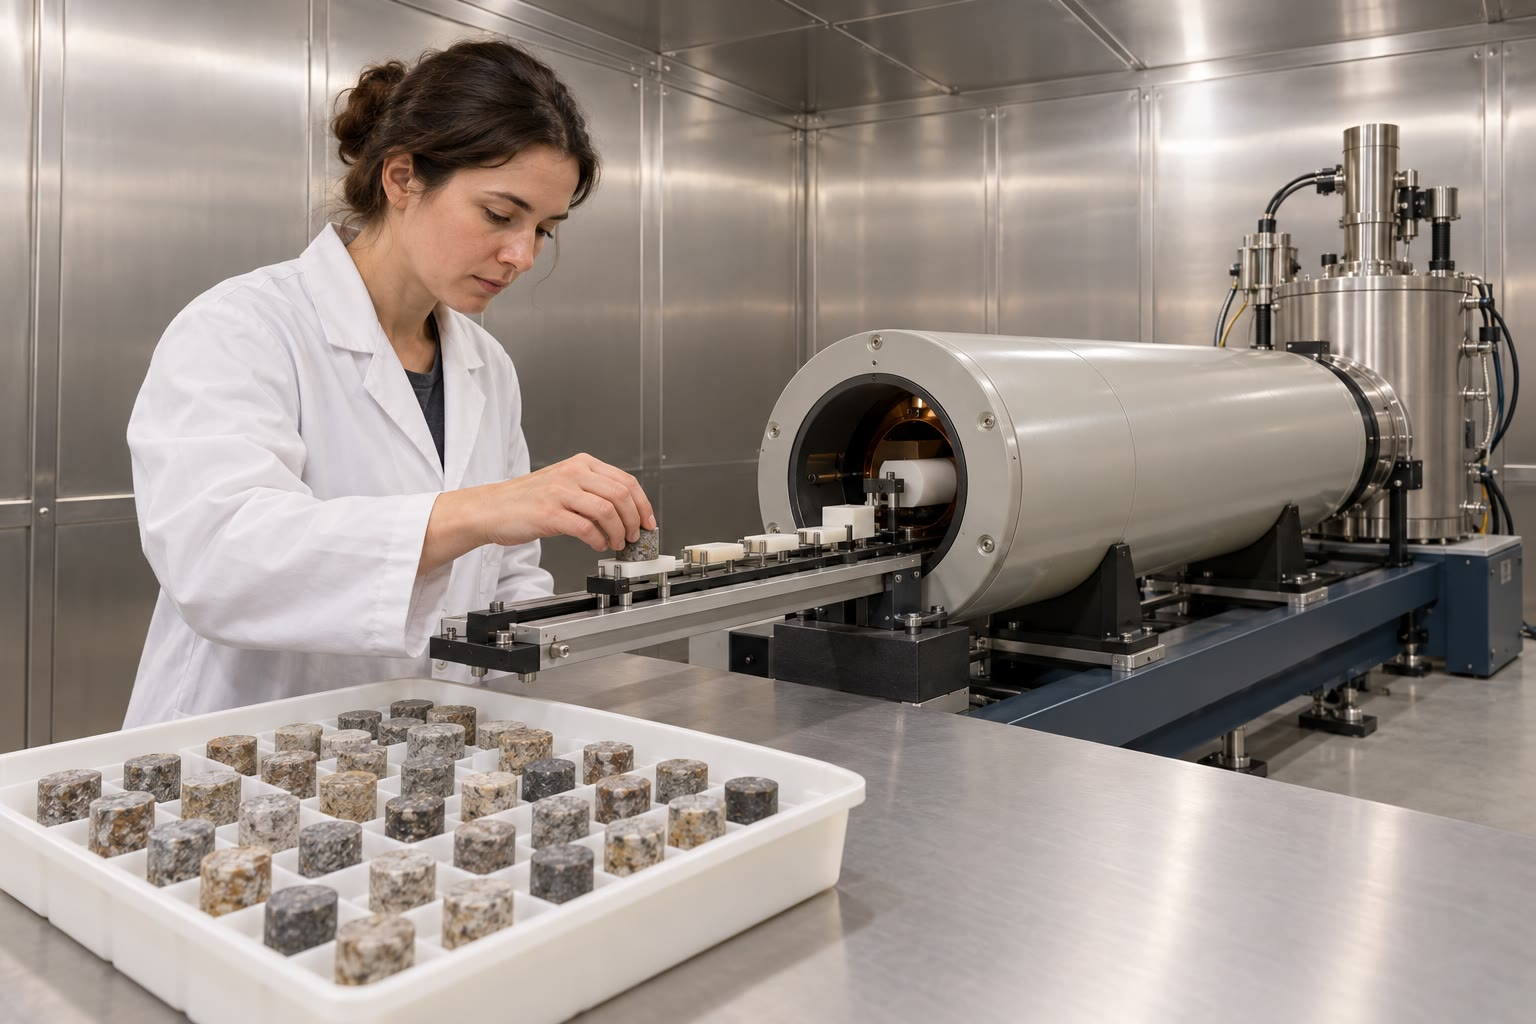
\includegraphics[width=\linewidth]{images/book5/ai/b3-palaeomag-lab.jpg}

{\scriptsize Loading specimens onto the sample tray of a magnetometer in a
shielded room (AI-generated illustration).}
\end{minipage}
\end{inthelab}

\section{Exercises}

\begin{exercise}[$\star$]\label{exo:b3:palaeomagnetism:1}
In a \omterm{def:b3:palaeomagnetism:main-field}{geocentric axial dipole} field, compute the inclination at latitude
\ang{30}\,N, and the latitude of a site where the inclination is \ang{-20}.
\end{exercise}

\begin{exercise}[$\star$]\label{exo:b3:palaeomagnetism:2}
At a station, the field has components $X = \qty{20000}{nT}$, $Y =
\qty{-2000}{nT}$ and $Z = \qty{40000}{nT}$. Compute $H$, $F$, the magnetic
declination and the inclination.
\end{exercise}

\begin{exercise}[$\star$]\label{exo:b3:palaeomagnetism:3}
In 2025, $g_1^0 = \qty{-29350}{nT}$. Taking the field as an axial dipole,
compute the field at the equator and at the poles, and the dipole moment
($a = \qty{6371.2}{km}$, $\mu_0 = 4\pi\times\qty{e-7}{H.m^{-1}}$).
\end{exercise}

\begin{exercise}[$\star$]\label{exo:b3:palaeomagnetism:4}
Name the kind of remanence acquired, and when it records the field, by: (a) a
lava flow cooling; (b) silt settling in a quiet lake; (c) a sandstone whose
iron oxide coatings turn to haematite during early burial; (d) a basalt sitting
for a million years in the present field.
\end{exercise}

\begin{exercise}[$\star\star$]\label{exo:b3:palaeomagnetism:5}
Four specimens of a site give the directions $(D, I)$: $(\ang{12}, \ang{48})$,
$(\ang{22}, \ang{44})$, $(\ang{16}, \ang{57})$ and $(\ang{6}, \ang{53})$.
Compute their unit vectors, the resultant length $R$, the mean direction, $k$
and $\alpha_{95}$.
\end{exercise}

\begin{exercise}[$\star\star$]\label{exo:b3:palaeomagnetism:6}
A site at \ang{40.0}\,N, \ang{10.0}\,E gives the mean direction $D = \ang{20}$,
$I = \ang{50}$. Compute its \omterm{def:b3:palaeomagnetism:vgp}{palaeolatitude} and its \omterm{def:b3:palaeomagnetism:vgp}{virtual geomagnetic pole}.
\end{exercise}

\begin{exercise}[$\star\star$]\label{exo:b3:palaeomagnetism:7}
The IGRF gives a dipole moment of \qty{8.32e22}{A.m^2} in 1900 and
\qty{7.69e22}{A.m^2} in 2025, and a rate of change of $g_1^0$ of
\qty{+12.6}{nT/yr} in 2025. (a) Compute the relative change of the moment per
century. (b) If $g_1^0$ kept that rate, in how many years would it reach zero?
Why is this not a forecast?
\end{exercise}

\begin{exercise}[$\star\star$]\label{exo:b3:palaeomagnetism:8}
A specimen's remaining remanence, in \unit{mA/m} (north, east, down), is
$(32.2, 18.1, 38.2)$ after heating to \qty{20}{\celsius}, $(25.8, 18.1, 24.6)$
after \qty{300}{\celsius}, and $(0.0, 0.0, 0.0)$ after \qty{580}{\celsius}; the
\omterm{def:b3:palaeomagnetism:zijderveld}{Zijderveld diagram} is straight between each pair. Compute the direction and
intensity of the component removed between 20 and \qty{300}{\celsius} and of
that removed above \qty{300}{\celsius}. Which is the ChRM, and what is the
other?
\end{exercise}

\begin{exercise}[$\star\star$]\label{exo:b3:palaeomagnetism:9}
A formation gives $I = \ang{-35}$ with $\alpha_{95} = \ang{5}$. Compute its
\omterm{def:b3:palaeomagnetism:vgp}{palaeolatitude}, the range of \omterm{def:b3:palaeomagnetism:vgp}{palaeolatitudes} allowed by $I \pm \alpha_{95}$,
and the semi-axes $\mathrm dp$ and $\mathrm dm$ of the confidence oval of its
pole.
\end{exercise}

\begin{exercise}[$\star\star\star$]\label{exo:b3:palaeomagnetism:10}
(a) From \cref{thm:b3:palaeomagnetism:dipole}, find the latitude where the
inclination is \ang{45}, and the ratio of the field at the poles to that at the
equator. (b) Show that $\mathrm dI/\mathrm d\lambda = 2/(1 + 3\sin^2\lambda)$,
and deduce where an error of inclination gives the largest error of
\omterm{def:b3:palaeomagnetism:vgp}{palaeolatitude}. (c) Why are \omterm{def:b3:palaeomagnetism:vgp}{palaeolatitudes} from low inclinations the most
precise in degrees?
\end{exercise}

\begin{exercise}[$\star\star\star$]\label{exo:b3:palaeomagnetism:11}
A site lies at \ang{35.0}\,S, \ang{150.0}\,E on a stable plate whose reference
pole, for the age of a formation sampled there, is at \ang{70.0}\,N,
\ang{300.0}\,E. (a) Compute the angular distance $p$ from the site to the pole,
the expected inclination and declination, and the expected \omterm{def:b3:palaeomagnetism:vgp}{palaeolatitude}.
(b) The formation gives $D_o = \ang{30.0}$, $I_o = \ang{-60.0}$. Compute the
rotation $R$ and the poleward displacement $P$, and say what they mean.
\end{exercise}

\begin{exercise}[$\star\star\star$]\label{exo:b3:palaeomagnetism:12}
(a) From \cref{prop:b3:palaeomagnetism:fisher}, show that the probability that
a direction lies within $\theta$ of the mean is $(e^\kappa -
e^{\kappa\cos\theta})/(e^\kappa - e^{-\kappa})$. (b) For large $\kappa$ and
small $\theta$, show that this is about $1 - e^{-\kappa\theta^2/2}$, and deduce
that \qty{63}{\percent} of the directions lie within $\theta_{63} \approx
\ang{81}/\sqrt\kappa$. (c) Compute $\theta_{63}$ for $\kappa = 50$, and check the
\qty{63}{\percent} with the exact formula.
\end{exercise}

\section{Problem: The Red Beds of Kesta}

\begin{problem}[{Weekend problem --- three formations of a displaced terrane,
their directions, poles and rotations, and the age of the youngest}]
\label{pb:b3:palaeomagnetism:1}
% values: calc/ch04.py; palaeomag_stats.py, magnetostratigraphy.py; GPTS: iodp:gpts2004
Kesta is an invented terrane, now at \ang{47.0}\,N, \ang{15.0}\,E, at the edge
of an invented stable continent. It exposes three red-bed formations: A,
\qty{60}{Ma}; B, \qty{30}{Ma}; C, from about 3.7 to \qty{2.4}{Ma}. Each was
sampled at several sites, and every specimen was thermally demagnetised; the
ChRM is carried by haematite, and the formations are horizontal.

\medskip\noindent\textbf{Part I --- Mean directions.} The six sites of
formation A give $(D, I)$: $(\ang{50}, \ang{37})$, $(\ang{28}, \ang{37})$,
$(\ang{21}, \ang{42})$, $(\ang{24}, \ang{27})$, $(\ang{37}, \ang{39})$,
$(\ang{46}, \ang{38})$.
\begin{enumerate}
  \item Why may a ChRM carried by haematite in a red bed be younger than the
        bed? What would show that it is not much younger?
  \item Compute the unit vector of the first direction.
  \item The six unit vectors sum to $(3.8943, 2.6500, 3.5717)$. Compute $R$ and
        the mean direction of formation A.
  \item Compute $k$ and $\alpha_{95}$ for formation A.
  \item Formation B gives, from 7 sites, $D = \ang{23.9}$, $I = \ang{51.5}$ and
        $R = 6.8979$; formation C, from 8 sites, $D = \ang{3.4}$, $I =
        \ang{63.7}$ and $R = 7.8707$. Compute $k$ and $\alpha_{95}$ of each.
  \item Which formation is the best grouped? Which mean is the best defined?
\end{enumerate}

\medskip\noindent\textbf{Part II --- Palaeolatitudes and poles.}
\begin{enumerate}[resume]
  \item Compute the \omterm{def:b3:palaeomagnetism:vgp}{palaeolatitudes} of A, B and C.
  \item For formation A, compute the palaeocolatitude $p$ and the latitude of
        its \omterm{def:b3:palaeomagnetism:vgp}{virtual geomagnetic pole}.
  \item Compute the longitude of that pole, checking which case of
        \cref{thm:b3:palaeomagnetism:pole} applies.
  \item Compute $\mathrm dp$ and $\mathrm dm$ for the pole of A.
  \item The poles of B and C are at \ang{66.5}\,N, \ang{135.6}\,E and
        \ang{87.1}\,N, \ang{139.1}\,E. Describe the path of the three poles
        with age.
\end{enumerate}

\medskip\noindent\textbf{Part III --- The age of formation C.} In formation C,
from its base, the specimens are reversed up to \qty{4.2}{m}, normal to
\qty{14.8}{m}, reversed to \qty{19.7}{m}, normal to \qty{24.6}{m}, reversed to
\qty{29.2}{m} and normal to \qty{54.0}{m}, then reversed to the top at
\qty{64.0}{m}. An ash bed at \qty{22}{m} is dated at about \qty{3.2}{Ma}. The
normal subchrons of chron C2An span 3.596--3.330, 3.207--3.116 and
3.032--\qty{2.581}{Ma}.
\begin{enumerate}[resume]
  \item Match the polarity zones with the timescale, using the ash bed.
  \item Compute the accumulation rate between the first and the third reversal
        boundary, and between the fourth and the sixth.
  \item Estimate the ages of the base and the top of the section.
  \item Why is the rate a mean over hundreds of thousands of years, and what
        could make it change?
\end{enumerate}

\medskip\noindent\textbf{Part IV --- Against the stable continent, and the drift.} The
reference poles of the stable continent are at \ang{78.0}\,N, \ang{190.0}\,E
($A_{95} = \ang{3.0}$) at \qty{60}{Ma}; \ang{83.5}\,N, \ang{175.0}\,E
($\ang{2.5}$) at \qty{30}{Ma}; and \ang{87.5}\,N, \ang{150.0}\,E ($\ang{2.0}$)
at \qty{4}{Ma}.
\begin{enumerate}[resume]
  \item Compute the angular distance from Kesta to the \qty{60}{Ma} reference
        pole, and the expected inclination and \omterm{def:b3:palaeomagnetism:vgp}{palaeolatitude}.
  \item Compute the expected declination at \qty{60}{Ma}.
  \item The expected directions at 30 and \qty{4}{Ma} are $(\ang{2.9},
        \ang{60.0})$ and $(\ang{2.5}, \ang{63.6})$. Compute the poleward
        displacement $P$ of A, B and C.
  \item Compute the rotation $R$ of A, B and C.
  \item Compute the errors $\Delta D_o$ and $\Delta D_x$ for A, and the error
        of its rotation.
  \item The errors of $R$ for B and C are \ang{13.8} and \ang{17.9}. Which
        rotations are significant at 95 per cent?
  \item Tell the history of Kesta relative to the stable continent.
  \item Compute Kesta's northward drift since formation A, with respect to
        the spin axis, in degrees and in kilometres
        (\qty{111.19}{km} per degree).
  \item Compute the \omterm{def:b3:palaeomagnetism:vgp}{palaeolatitudes} allowed by $I \pm \alpha_{95}$ for
        formation A, and take as one standard deviation half the width of that
        interval divided by 1.96. Give Kesta's northward drift since formation
        A, in kilometres, with its standard deviation.
\end{enumerate}
\end{problem}
